\documentclass[class=article, crop=false]{standalone}
\usepackage[subpreambles=true]{standalone}
\usepackage{zk}

\usepackage{graphicx}

\externaldocument[per-0021-]{per-0021}
\externaldocument[per-0018-]{per-0018}

\begin{document}

\makeheader[A summary of paradata encompassing definition, historical background, how paradata gets generated, the various types of paradata, use cases of paradata, and the future (as well as concerns) of paradata.\keywords{overview, paradata, definition, background, examples, use cases}]{Overview of Paradata}\label{first}

\section{Definition of Paradata}
\label{first}
\keywords{paradata, definition}

The simplest definition of paradata is that it is ``data about processes''. \cite{huvilaPerspectivesParadataResearch2024}
Paradata seeks to capture the ways in which information comes or came to be.
The InterPARES Project expands the definition more broadly but is oriented around this simplified definition \cite{davet2022tracking}:

\begin{displayquote}
Information about procedures and tools used to create and process information resources, along with information about the persons carrying out those procedures.
\end{displayquote}

Adding to the problematic nature of rigorously defining paradata is that paradata is often left undocumented or implicit within data sources. \cite{borjesson2022re,huvila2021documenting}
This can partially be due to paradata itself being a vague concept where there is a ``certain amount of chaos'' in the management and defining of paradata. \cite{cohen2024paradata}
As a result, using simpler definitions such as ``data about processes'' can ameliorate some of the concern about ``what'' exactly is paradata - at the cost of precision.

\printbib

\section{Background on Paradata}
\label{first}

Paradata draws attention to the invisible knowledge of processes. \cite{prusak2001did}
It makes one aware of the history and future of information and how that information came into existence.
It aids in surfacing and understanding processes while highlighting the invisible conscious or unconscious decisions involved within processes.
In other words, paradata makes tacit knowledge (i.e. practices) about a process a "known unknown". \cite{huggett2020capturing}

Additionally, while paradata is a technical description, processes come into existence at the intersection of a variety of factors.
Specifically, processes themselves are sociotechnical objects.
They are built using physical and digital architecture and formed by the needs people and organizations impose upon them \cite{bowker2000sorting,dourish2022stuff,hine2006databases}
In this way, paradata may serve as a tool for reflection on a process's reliability, validity, and reproducibility across contexts.

\section{Examples of Where Paradata May Be Generated }
\label{first}

In general, paradata is created while collecting and/or analyzing data. \cite{o2017secondary,schenk2024paradata}
Paradata, whether intentionally recorded or not, can be created in meeting minutes, in a researcher's private notes, or in project reports.
Additionally, project or research paradata can be found where researchers share the status of their efforts such as at conferences or in conference posters. \cite{huvilaPerspectivesParadataResearch2024}

\subsection{Survey Instruments}

Specifically and historically, one of the earliest places where paradata was first explicitly described and delineated was in the context of qualitative interviews and survey methodologies.
In these situations, paradata such as mouse movement information and keystroke response time data could be collected and have become objects of research in their respective fields. \cite{fahmy2017using}

\subsection{Datasets}

More recently, paradata can also appear routinely within exploratory data analysis of datasets and databases.
In this context, this would be paradata that details progress in exploring or using a particular dataset.
Moreover, paradata can continuously be developed when working with a dataset as a researcher continues to either become more familiar with the data or needs evolve.
Some paradata examples could be recording the way to extract from the dataset particular subsets of data or software or techniques with how best to work with the dataset. 


\section{Types of Paradata}
\label{first}

Paradata needs overlap and can require multiple paradata types to understand a dataset.
Many different types of paradata are described in, \cite{huvilaPerspectivesParadataResearch2024} and are listed below:

\subsection{Scope Paradata: What Does the Data Cover}
\label{first}

Scope paradata addresses information needs relating to data reuse.
In particular, it highlights what available data does and does not cover.

\subsection{Provenance Paradata: Where Does Data Come From}
\label{first}

Provenance paradata categorizes information along disciplinary and timebound origin, epistemological culture, and the rationale of data generation.
Beyond the rationale of how data was generated, this data communicates the moment in history of how a discipline conducted itself or interpreted research materials.

\subsection{Methods Paradata: How Data Was Generated}
\label{first}

Methods paradata explores the procedures in data generation.
It concerns research methods, information on techniques and decision-making.

\subsection{Knowledge Organization and Representation Paradata: How Data Is Structured and Communicated}
\label{first}

Knowledge organization and representation paradata concerns how data is structured, categorized, and communicated, providing insights into the frameworks and systems shaping the data’s meaning.


\subsection{Survey Instruments}

Paradata has even been used as the basis for machine-learning-based predictive analyses \cite{fernandez2020predicting}

\subsection{Databases}

“This leaves the “new” collection manager with the unenviable task of reverse engineering a database’s structure, contents, and data entry workflows for the next generation. Even once reverse engineered, not knowing the reasons underlying database design decisions makes database usage difficult” \cite{rayburn2024reconstructing}

\textit{
  NOTE: There is probably a story to explore about how paradata could help with database migrations and updates between database schema versions. 
}

\subsection{Sources To Investigate}

I don't have time to check these sources out, but there could probably be some interesting insights here to be had from:

\begin{itemize}
  \item \href{https://journals.sagepub.com/doi/full/10.1177/08944393211032950}{Predicting respondent difficulty in web surveys: A machine-learning approach based on mouse movement features} 

  \item \textit{Working with Paradata, Marginalia and Fieldnotes} - Chapter 3
\end{itemize}


\section{Future and Concerns around Paradata}
\label{first}

It has often been noticed that while recording and managing paradata is and can also be useful, it can be conceptually difficult to define and intensive to record.
This is due to the strongly interdisciplinary and/or intersectional nature of paradata emerging at the "interface between practices, processes, and their related entities.” \cite{huvilaPerspectivesParadataResearch2024}

As notions related to paradata continue to become concretized, emerging schools of thought around paradata's place in the landscape of information have also emerged.
To highlight two emerging ethics there is the notion of paradata as describing "the relationship between science and social justice" and the other seeing paradata as the means to communicate "clean data and accuracy as an ethical issue" itself. \cite{mickel2023cultural}
In particular, these two emerging schools of thought are not at odds with one another and are actually strongly compatible and even complementary.
Moreover, there can be outright immoral or dangerous motivations to generate or control the record of certain paradata.
As pointed out by \cite{huvilaPerspectivesParadataResearch2024}, there can be misuse of paradata such as:

\begin{itemize}

  \item Conveniently leave out or misrepresent the actual process information that went into making a particular process decision or process overall.

  \item Attribute complexity of a process's paradata as "necessary" when in fact the process is just poorly made and implemented.

  \item Control the perception of a perfectly good or even better process in order to discount or discredit it.

\end{itemize}


I appreciated \nameref{per-0018-first}'s thoughts here on thinking about the limitations around paradata.
I felt like they were very practical and at the same time agenda setting for the practicalities of paradata in practice.
\nameref{per-0018-first} pointed out some promising ideas being:

\begin{itemize}
  \item Homogenisation for known uses 
  \item Systematisation of basic data structures with an option to extend them
  \item Description of vocabularies
  \begin{itemize}
    \item Thesauri, terminologies, word lists, descriptionss of terms
  \end{itemize}
  \item Documentation of knowledge organisation and knowledge representation
  \item Description of silent knowledge of "how things are done"
  \item Description of anomalies
\end{itemize}

At the same time, \nameref{per-0018-first} pointed out some hazardous pitfalls when working with paradata:

\begin{itemize}
  \item Homogenisation with a clear aim
  \item Systematisation of how knowledge should or must be represented
  \item Systematisation of what knowledge can be created
  \item Cleaning for the sake of cleaning
  \item Forced templates AP
  \item Overdocumentation
  \item Belief in that all can/must be documented
\end{itemize}


\section{Data Makers and Users' Views on Useful Paradata: Priorities in Documenting Data Creation, Curation, Manipulation and Use in Archaeology}
\label{first}
\keywords{reference, paper, paradata, archaeology}

While this paper didn't reveal much more information to me, I did really appreciate how they assessed researcher and administrator care about paradata.
I think it could be extremely useful as inspiration for conducting research into paradata for other fields.

The following table shows how they assessed individuals for all sorts of questions on what they care about most with paradata in the context of archaeology.

\begin{figure}[h!]

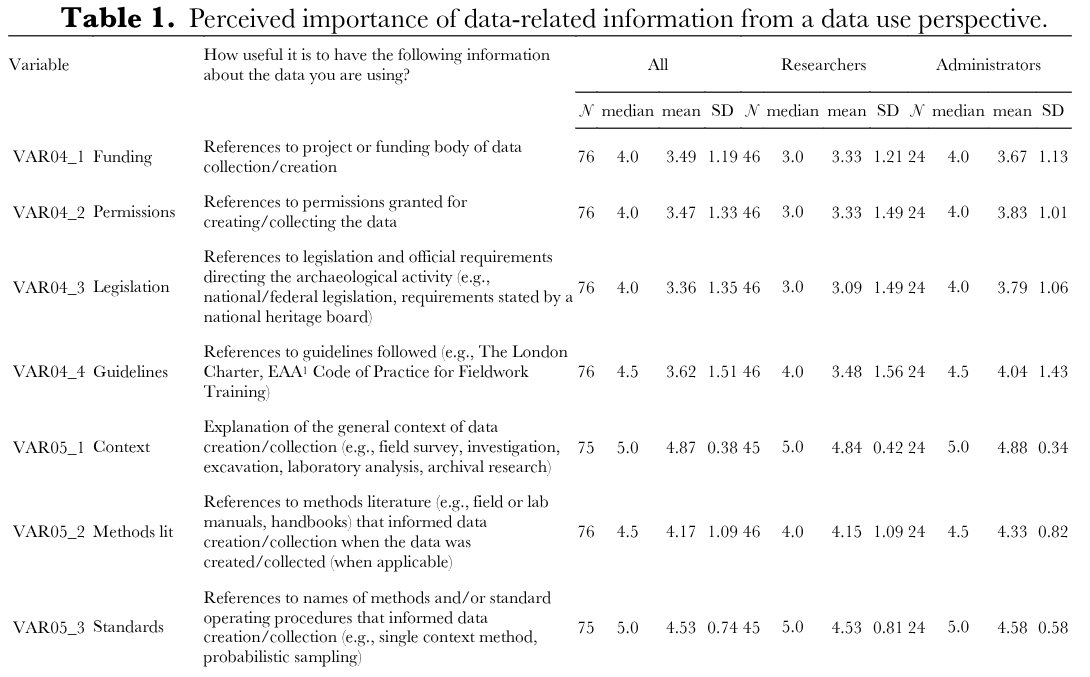
\includegraphics[width=\textwidth]{data_question_table.jpg}
\caption{}

\label{tab:data-question-table}

\end{figure}


\section{Random Thoughts and Insights about Understanding Paradata}
\label{first}
\keywords{paradata, thoughts}

These are just random thoughts I have had both from myself and from colleagues about paradata.
As paradata is still such a new idea, there is plenty to latch on here and translating it to other domains.
Might be some nuggets in here, might not be while ideas develop.

\subsection{Discussion with \nameref{per-0021-first}}
\label{second}

\nameref{per-0021-first} suggested that there is quite some similarity between paradata and \href{https://en.wikipedia.org/wiki/Traceability_matrix?useskin=vector}{Traceability Matrices}.
I am not quite sure but with \nameref{per-0021-first}'s experience as a human systems engineer, there has to be something here.
 
\printbibliography

\end{document}
